\section{Solver Quality Definition and Calculation} \label{sec:SQ}

%%\nisar{note to self: stopped here...also need to improve technical description: use more conventional phrasing like `surrogate function/model' to describe what is going on with the trusted solver...some of this is used later, but should be used here}

The insights above are extended to formally define and compute the solver quality \famsec{} factor \xQ{}. In the context of APS planning, \xQ{} indicates how well a generic solver \solve{} for a planning problem will `perform' on a given task \task{} of class \taskclass{}. This work restricts \taskclass{} to the class of all applicable MDP problems, so that \solve{} is any type of MDP solver  (although the ideas developed here can in principle be easily extended beyond MDPs or planning problems alone). %%...(or for that matter, a planner for any other problem type, or APS algorithm for any other APS capability)


A formal definition for \xQ{} must make the notion of \solve{}'s `performance' precise to enable some form of quantitative evaluation. For MDPs, any particular task instance \task{} has a corresponding optimal policy \piopt{} which by definition leads to corresponding best achievable total reward. This suggests that a natural performance metric for assessing the competence of a generic solver \solve{} would be some quantitative comparison of the (approximate) policy \piapprox{} to \piopt. Such a `strong' comparison can be done in many ways depending on the application context, e.g. by directly comparing actions taken by the policies in different states of interest, or by comparing the resulting expected total reward distributions or other artifacts of the different policies. 
But since \piopt{} is usually unavailable (or else \solve{} would not be needed), \xQ{} should also allow for `weak' comparison to other reference `baseline' solvers that yield policies with performance as good as/very close to the true optimal \piopt. This may require comparing two completely different types of solvers (e.g. a deterministic approximation vs. a Monte Carlo approximation), so \xQ{} should also ideally enable comparison across solver classes, as well as assessments of online/anytime solvers (for which complete state coverage and policy convergence may not be possible in large state/action spaces). %%\nisar{--large state spaces which necessitate use of approximate policies might make comparison of converged approximate solution infeasible, so must further allow for assessment/comparison of anytime/good enough results (i.e. strict convergence or coverage of full state space not required...)}

%%\nisar{For RSS: we should formalize this notion in terms of `strong' performance comparison w.r.t. true exact optimal policy, and `weak' performance comparison w.r.t. reference/baseline solver (which notionally in our case should produce policies as good as/close to true optimal, or at least have properties that allow it to converge...) }
 
At the same time, \xQ{} should account for the expected self-confidence metric trends and boundary conditions mentioned earlier in Fig. \ref{fig:trendsBCs} for the Donut Delivery application. In particular, \xQ{} should be defined also to naturally account for the influence of both characteristics of \solve{} and features of \task{} simultaneously. For instance, if the task \task{} is not particularly complex or is characterized by a very small amount of uncertainty (e.g. so as to be nearly deterministic), then it is possible that a small sample size could suffice to closely approximate the optimal policy, in which case \xQ{} should indicate very high confidence. Moreover, while it is impossible to assess performance on \emph{all} tasks in \taskclass{}, \xQ{} should be able to reflect \solve{}'s performance on \emph{any} task instance \task{} in \taskclass{}, including previously unseen tasks (e.g. new road networks for the Donut Delivery problem). 
%\nisar{...It is generally impossible to evaluate the exact solution for \emph{all} tasks of a given task class \taskclass{} -- weak/strong again: weak is for any given task, strong is for all possible tasks...}

%\xQ{} would generally be expected to reflect decreased confidence for a Monte Carlo-based solver as the number of samples used to approximate the optimal policy $\pi$ decreases, since the state space for \task{} will be less thoroughly explored. However, if the task \task{} is not particularly complex or is characterized by a very small amount of uncertainty (e.g. so as to be nearly deterministic), then it is possible that a small sample size could suffice to closely approximate the optimal policy, in which case \xQ{} should indicate very high confidence. Therefore, 

%\nisar{this should be stated more precisely: how closely the policy produced by a solver \solve{} approximates an optimal/baseline policy or how well it performs relative to an optimal/baseline policy...there is a nuance here in the choice of comparing policies vs. value functions/total expected reward, which is alluded to below but not clearly stated as such...}
%(i.e. all road networks with a , , and exit, et cetera as described previously). 
%The need for \xQ{} is not necessarily easy to understand; an analogy helps to clarify: \brett{I have now started thinking about \xP{} being the \emph{shape} of the distribution, and \xQ{} referring to the location of the distribution with respect to the trusted \solvestar{}}
%
%\emph{Clarifying Example:} One could informally think of \xQ{} as an indication of the \emph{ability} of an athlete. This is opposed to the athlete's assessment of the desirability of the outcome of a game (\xO). While an athlete may be very capable (high \xQ), the score of the game may be such that the athlete knows that it is nearly impossible to catch up and win the game (low \xO). Conversely, an athlete may not be very capable (low \xQ), and due to being na\"{i}ve has an incorrect assessment of the desirability of the outcome (\xO{} cannot be trusted). \nisar{might be best to put this at end/conclusions somewhere to highlight future directions and connections...}
    
%The formal desiderata for \xQ{} are: (\textbf{D1}) reflect competence of solver \solve{} for task \task{}; (\textbf{D2}) enable comparison across solver classes; (\textbf{D3}) extend to unseen tasks of the same class. 
    %\begin{enumerate}[label=\textbf{D\arabic*}]
    %    \item reflect competence of solver \solve{} for task \task{} (where competence is analogous to the `ability' of the athlete in the example)\label{itm:d1}
    %    \item enable comparison across solver classes \label{itm:d2}
    %    \item extend to unseen tasks of the same class \taskclass \label{itm:d3}
    %\end{enumerate}
%    
%For practical application, it is critical to be able to compare the quality of solvers of different classes (i.e. exact vs. approximate) because there are many different ways of solving tasks. Likewise, it is also common for an APS to encounter a similar, but previously unseen, task (i.e. a different road network).
%    
%\nisar{this should come earlier and be more technically precise/clear...no sense in talking about competence and quality for a few parags if these are not defined up front!} 

%Evaluating the `quality' of something implies some kind of comparison is taking place. In this setting the desired comparison is between a `candidate solver' \solve{} and some reference solver. Ideally, the candidate solver could be compared to the exact solution (whose quality is by definition perfect), but there are three main challenges: 1) It is unclear how policies/solvers should be compared; 2) Large state spaces make exact solutions infeasible; and 3) It is generally impossible to evaluate the exact solution for \emph{all} tasks of a given task class \taskclass{} (linked to \ref{itm:d3})
    
%\nisar{use to extend previous parag and transition to next subsubsection...need to close the loop and remark on how our approach neatly checks off all the boxes above...}   
 %A natural starting point for this is: what information related to the assessment of \xO{} can also be used to directly inform \xQ{}? 
 A natural starting point for devising a quantitative assessment of \xQ{} according to these desiderata is to again examine how information about $\rwd=\pri$ (which is already used to form \xO{}) can be analyzed further. 
 Note that \xO{} indirectly depends on \xQ{}, since reliable estimation of \rwd{} requires knowing \piopt. But in practice, an MDP-based APS will often employ an approximate policy \piapprox{} instead of the true optimal policy \piopt. In turn, this leads to an estimate \ppiapproxri{} of the expected reward distribution which differs from the true \ppioptri{} under the optimal \piopt. We show next that, if a surrogate model for \rwdpredicted{} for \rwdtrust{} can be found when \piopt{} is unknown but \pitrust{} is available (where $\pitrust \approx \piopt$), then a quantitative comparison of the simulated \rwdcandsim{} of a `candidate' solver to the surrogate \rwdpredicted{} leads to a suitable metric for \xQ{} (under the progressively relaxed assumption of \xM{}=\xMup, \xP{}=\xPup, and \xI{}=\xIup). 
    
        %
    % \subsubsection{Summary} The comparison of policies will be done through comparing reward distributions; this approach addresses both \ref{itm:d1} and \ref{itm:d2}, along with \ref{itm:l1}. In order to address \ref{itm:l2}, \ref{itm:l3}, and \ref{itm:d3} a `trusted solver' \solvestar{} will be introduced to serve as a basis by which a `candidate solver' \solve{} can be evaluated. Furthermore, a surrogate model \surrogate{} will be learned to predict \rwdstarapprox{} on un-encountered tasks. In this way, all desiderata, and challenges have been addressed.
    
    % \begin{figure}[tb]
    %     \centering
    %     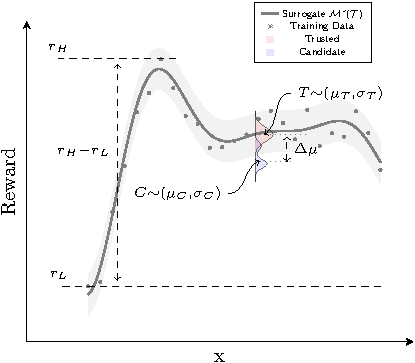
\includegraphics[width=0.55\linewidth]{Figures/sq_v2_fig-crop}
    %     \caption{Key values involved in calculating \xQ, where $x$ represents a `parameter of interest' for task \task, or solver \solve.}
    %     \label{fig:sq_v2}
    %     \vspace{-0.2cm}
    % \end{figure}
    
       \begin{figure}[tb]
        \centering
        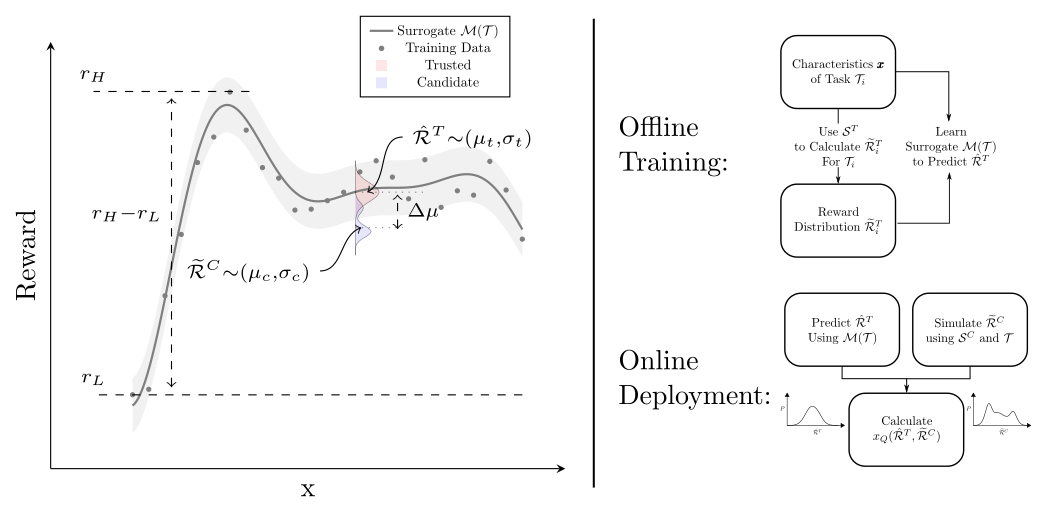
\includegraphics[width=0.79\linewidth]{Figures/xQ_combined.png}
        \caption{(Left) Key values for computing \xQ, where $x$ is a `feature of interest' for \task or \solve; (right) offline training phase of surrogate \surrogate{} and online calculation of \xQ{}. }
        \label{fig:sq_v3}
        \vspace{-0.2cm}
    \end{figure}
\input{"methodology.tex"}    
